\section{Modelo de Dados}\label{sec31}

%
% Base de Dados
%
\subsection{Base de Dados}\label{subsec311}

Os dados são armazenados de forma persistente numa \acrfull{bd}. A \acrshort{bd} utilizada é relacional uma vez que não se preveem alterações ao esquema das tabelas, não carecendo do dinamismo oferecido por uma \acrshort{bd} documental, por exemplo. 

A escolha de qual o melhor \acrfull{sgbd} assentava em três possibilidades, \textit{SQL Server}, \textit{PostgreSQL} e \textit{MySQL}. O primeiro apesar de ser uma ferramenta com a qual o grupo estava familiarizado foi automaticamente excluído visto que um dos requisitos pretendidos era usar ferramentas \gls{open-source}, caraterística não presente neste sistema. Os restantes sistemas são \gls{open-source} e têm uma elevada compatibilidade com os principais fornecedores de serviços \textit{cloud}. Pelo que a verdadeira distinção se prende com as vantagens oferecidas pelo sistema \textit{PostgreSQL}:
\begin{itemize}
	\item O \textit{PostgreSQL} é compatível com as propriedades \acrfull{acid}, garantindo assim que todos os requisitos sejam atendidos;
	\item O \textit{PostgreSQL} aborda a concorrência de uma forma eficiente com a sua implementação de \acrfull{mvcc}, que alcança níveis muito altos de concorrência;
	\item O \textit{PostgreSQL} possui vários recursos dedicados à extensibilidade. É possível adicionar novos tipos, novas funções, novos tipos de índice, etc.
\end{itemize}
Assim sendo, foi escolhido o \acrfull{sgbdro} \textit{PostgreSQL}, como já anteriormente mencionado, na secção \ref{subsec233} do capítulo \ref{cap2}.

\subsubsection{Implementação}\label{subsubsec3111}

Na \acrshort{bd} foram desenvolvidas funções que garantem a consistência dos dados, por um lado na inserção de entidades cujos \textit{IDs} sejam incrementais ou gerados consoante o desejado, por outro lado na remoção  de entidades que se relacionam com outras.

Decidiu-se usar funções na \acrshort{bd} em vez de criar métodos em \textit{Java}, pois se imaginarmos um cenário onde a aplicação servidora esteja distribuída, existe um problema no controlo da concorrência na geração dos \textit{ID}s. Tendo em conta que a \acrshort{bd} não é distribuída então o problema descrito não existe.

% Modelo EA
\subsection{Modelo Entidade-Associação}\label{subsec312}

\begin{figure}
%	\hspace*{-2,5cm}
	\centering
	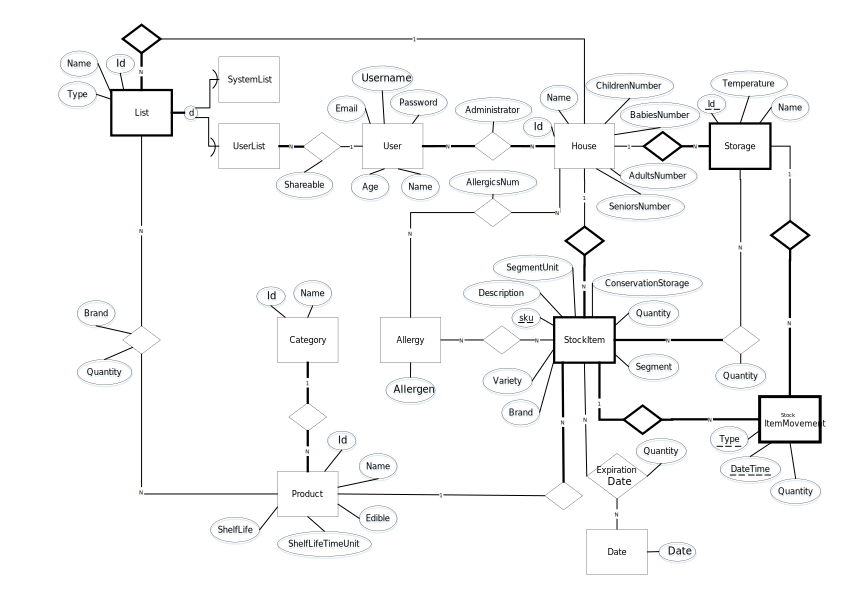
\includegraphics[width=1\textwidth,scale=1,trim={5mm 5mm 5mm 5mm},clip]{img/EA.pdf}
	\caption{Modelo Entidade-Associação}
	\label{modelo-ea}
\end{figure}

Com Figura \ref{modelo-ea} é possível entender as relações das entidades referidas na secção \ref{sec24} do capítulo \ref{cap2}. Para um maior detalhe do domínio de cada uma das entidades consultar o anexo \ref{seca11}. 


\subsection{Particularidades do Modelo de Dados}

\subsubsection{Alergias dos Membros de uma Casa}

O sistema Smart Stocks disponibiliza um leque de funcionalidades, porém o foco do projeto prendeu-se com a parte relativa à gestão de stocks, deixando a parte da administração de casas e utilizadores para segundo plano. Contudo pensaram-se em alternativas, para implementar no futuro, que permitam que a gestão de utilizadores e casas seja mais pessoal e funcional. 

Um dos aspetos a ter em conta, seria a manutenção da consistência das alergias numa casa, aquando um utilizador é removido desta. Este aspeto é importante, pois o modelo de dados desenvolvido não garante essa coerência, visto que as alergias estão associadas a uma casa e aos seus membros e não a um utilizador do sistema. Tomou-se esta decisão, uma vez que faria mais sentido, na altura, as alergias estarem associadas a uma casa e ao seu conjunto de membros, que podem ou não estar registados no sistema. A razão desta escolha baseia-se na possibilidade de registar as alergias dos co-habitantes da casa, mesmo que estes não sejam utilizadores do sistema. 

Um bom exemplo que apoia esta abordagem, é o caso das crianças, desta forma, os seus pais registam as alergias dos mais pequenos e conseguem melhor controlar o plano alimentar familiar. Imagine-se uma casa com três habitantes, dois dos quais intolerantes à lactose, e apenas um está registado no sistema. O contra da solução é não saber qual dos membros detém a alergia, todavia, sabe-se que a mesma existe e assim é possível alertar o utilizador do sistema. Para concluir, esta solução apesar das suas vantagens, está acompanhada de um problema, que é a saída de alguém da casa, ficando a informação relativa às alergias inconsistente. Uma possível solução passa por notificar o administrador da casa para esse facto, e alertá-lo para a necessidade de retificar os dados.

\subsubsection{Internacionalização}

A internacionalização não é suportada ao nível da base de dados, não tendo por tanto tradução das nomenclaturas das categorias nem dos produtos, nem qualquer informação destes.  

